% -----------------------------------------------------------
\subsection{Analysis of Rewards \& Penalties}
% -----------------------------------------------------------
\subsubsection{Rewards}
% ------------------------------------------------
Elowsson (2024) published a comprehensive post on ethresear.ch on Ethereum issuance. This post included analysis and modelling of consensus incentives and variability of solo staker reward, as well as several other aspects relevant to issuance and staker yield (\href{https://ethresear.ch/t/properties-of-issuance-level-consensus-incentives-and-variability-across-potential-reward-curves/18448}{Properties of issuance level: consensus incentives and variability across potential reward curves}).

Note that rewards earned by a compounding validator does not need to pass through the activation churn due to the small amounts of ETH involved (in conversation with Mikhail). \\ 

\noindent
\textbf{Proposer rewards} \\
% ------------------------------------------------

\noindent
\textit{Proposer award for attestations} \\
% ------------------------------------------------


\noindent
\textit{Proposer award for sync committees} \\
% ------------------------------------------------




\noindent
\textbf{Attestation rewards} \\
% ------------------------------------------------



\noindent
\textbf{Whistleblower reward} \\
% ------------------------------------------------


\noindent
\textbf{Sync committee rewards} \\
% --------------------------------------------
A sync committee of 512 members is selected from the active validator every 256 epochs. To become a member, the next validator selected from a shuffled index is checked to see if it passes the sync membership test. The entire validator set is shuffled every time before another validator is drawn randomly from the set. Therefore, validators may be selected more than once, but this rarely happens when the validator set is very large, as is currently the case ($\sim$ 900,000 in January 2024).

The per-epoch reward for each sync committee member that performs its duties correctly during that epoch is calculated as follows: 


``Sync committee participants receive a reward for every slot that they correctly perform their duties. With 512 members in the committee, and 32 slots per epoch, the reward per validator per slot for correct participation is


There is the total increments of the whole active validator set, so this is a large number. The per-epoch per-validator reward is 32 times this.

The maximum issuance per epoch to sync committee members in respect of their sync contributions is then''


% ------------------------------------------------
\subsubsection{Penalties}
% ------------------------------------------------
% ------------------------------------------------
\textbf{Slashing penalties} \\
% ------------------------------------------------
\noindent
Listed below are links to posts about slashing penalties, the effect on them when EIP-7521 is implemented, including some proposals for modifications to existing penalties:
\begin{enumerate}
\item \href{https://a16zcrypto.com/posts/article/the-cryptoeconomics-of-slashing/}{The cryptoeconomics of slashing} by Kannan and Deb.
\item \href{https://ethresear.ch/t/slashing-penalty-analysis-eip-7251/16509}{Slashing penalty analysis} by Neuder and Monnot.
\item \href{https://notes.ethereum.org/@mikeneuder/slashings-eip-7251}{DRAFT] Slashing penalty analysis; EIP-7251} by Neuder and Monnot.
\item \href{https://hackmd.io/@dapplion/maxeb_slashing_risks}{MaxEB slashing risks} by dapplion
\item \href{https://colab.research.google.com/drive/1lBe4qH4oqI8D9cmcQGca3O1AdR3SVr5z?usp=sharing#scrollTo=Hiw1NPEZIQVi}{Slashing simulation code}
\end{enumerate}


\noindent
In the $3^{rd}$ blogpost, Neuder and Monnot propose the following for current slashing penalties \cite{Neuder2023d}: 
\begin{itemize}
\item Changes to existing penalties:
	\begin{itemize}
	\item Changing the \textit{initial penalty} to be either fixed, or scaled sublinearly
	\item Changing the \textit{correlation penalty} to scale quadratically rather than linearly.
	\end{itemize}
\item Unchanged penalties:
	\begin{itemize}
	\item \textit{Attestation penalties}
	\item \textit{Inactivity leak penalties}
	\end{itemize}
\end{itemize}

\noindent
\textbf{\textit{Initial slashing penalty}} \\
% -------------------------------------------------
The initial slashing penalty is proportional to the validator's effective balance, $MIN\_SLASHING\_PENALTY\_QUOTIENT\_BELLATRIX=32$, giving a maximum penalty of 1 ETH if the slashed validator has 32 ETH, the current MaxEB.
If left unchanged, a fully consolidated validator would incur an initial slashing penalty of 64 ETH. There appears to be general agreement that this initial penalty is too high, and may deter larger stakers such as Lido to support EIP-7521.

Neuder and Monnot suggest that the initial penalty could either be changed to a constant value, or through a monotonically increasing function, e.g.  from the family of polynomials. The latter appears to be the preferred option. However, mention has also been made of a zero initial slashing penalty since a slashed validator already incurs additional penalties such as attestation penalties and lost revenue while waiting for its exit epoch. Francesco is not in favour of a zero initial penalty because that means that there is no penalty to proposal equivocation, which is already a relatively cheap \gls{dos} attack vector on the network. For example, it is not good if someone can make 1,000 different blocks at zero cost.

For a monotonically increasing function, the authors propose the following function to calculate the revised initial slashing penalty:\\
\textit{initial penalty =} $\frac{EB^x}{32}, \texttt{ } x \leqslant 1$ \\

Their blogpost has graphs for $x=1, \frac{15}{16}, \frac{7}{8}, \frac{3}{4}, \frac{1}{2}$ and a line for a constant initial penalty of 1 ETH \cite{Neuder2023d}.

The authors conclude that visually it appears that $x = \frac{3}{4}$ and $\frac{7}{8}$ are good choices in terms of balancing the size of the initial slashing penalty and the risk for a consolidated validator.\\

Since the previous discussion and reasoning, an alternative point of view has been put forward, and that is to set the initial slashing penalty to zero. LIDO appears in favour of a small penalty as a deterrent, but penalties are already incurred due to the enforced wait time to the exit epoch and a small or zero initial penalty would not seem all that relevant. Moreover, a zero initial slashing penalty would favour smaller stakers over larger stakers.

Lion commented that setting the initial slashing penalty to zero does not fix the original aim of splitting attester and proposer slashing.  Although not specifically related to MaxEB, Lion summarised discussion around proposer and attester slashing in the following \href{https://docs.google.com/document/d/1mOc5nokVm3jx4bCffTuQ_xjYV4zVlDLPI-KEhFWWP78/edit}{blog post}.

\noindent
\textbf{\textit{Correlation penalty}} \\
% --------------------------------------------
This penalty is incurred roughly 18 days (4,096 epochs) after the slashing event, half way between its exit epoch and the slashing event \cite{Edgington2023}. The correlation penalty is important in penalising apparent coordinated attacks on the chain, and is the only other penalty that Neuder and Monnot propose to alter \cite{Neuder2023d}.

The penalty for a slashed validator is calculated as follows using the previous 36 days from this ``half-way'' epoch.
\begin{equation*}
\begin{split}
& \textit{correlation penalty} = \left\lfloor \frac{3*EB*SB}{TB} \right\rfloor, \texttt{ } where \\
& 3 = \textit{Bellatrix multiplier} \\
& EB = \textit{slashed validator's effective balance} \\
& SB = \textit{total slashable balance} \\
& TB = \textit{total effective balance of the beacon chain} \\
& \therefore \textit{if SB} = \frac{1}{3} * TB \implies \textit{ correlation penalty} = EB \\
& \textit{Similarly, if } 3*EB*SB <  TB \implies penalty = 0 \textit{ due to integer division} \\
\end{split}
\end{equation*}

There is currently no correlation penalty for isolated slashing events and this continues to be the case for a fully consolidated validator with 2,048 ETH effective balance as shown below using 24 million ETH as the total staked ETH, (\textit{TB}):

\begin{equation*}
\begin{split}
& \textit{ SB = EB for an isolated slashing} \\
& \therefore  3*EB*SB =  3*EB*EB \\
& \textit{Assuming EB = 2,048 \& TB } = 2.4 * 10^7, \textit{ then} \\
& 3*EB*EB = 1.2582912 * 10^7 < 2.4 * 10^7 \\
& \therefore penalty = 0
\end{split}
\end{equation*}

For EIP-7521 the authors propose a function that preserves the requirement that when the total slashed balance is $\frac{1}{3}^{rd}$ of the total balance, the entire balance of the validator is slashed:

\begin{equation*}
\begin{split}
& penalty' = \frac{3^2 * EB * SB^2}{TB^2} \\
& \therefore \textit{if SB } = \frac{TB}{3}, \textit{ then} \\
& penalty' =   \frac{3^2 * EB * \left(  \frac{TB}{3} \right)^2 }{TB^2} \\
& \therefore penalty' = EB
\end{split}
\end{equation*}

Moreover, the new correlation penalty function scales quadratically as opposed to the current function that scales linearly. With the proposed new function, the slashing penalties are substantially reduced for all validators, regardless of whether they have consolidated stake.

Refer to the \href{https://notes.ethereum.org/@mikeneuder/slashings-eip-7251}{blogpost} to view graphs showing the comparative correlated slashing penalties for solo (32 ETH), partially consolidated (256 ETH), and fully consolidated (2,048 ETH) validators applying both the current and the proposed functions \cite{Neuder2023d}. \\

Lion summarised some discussion around proposer and attester slashing, with the aim of decoupling correlated penalties from equivocating proposers and reducing a validator's time in exit status. (\href{https://hackmd.io/@dapplion/S1pGYKR_T}{blog post}). Independence is required for message replay protection. By reverting this \gls{pr} consolidated validators have a higher expected cost of proposer errors. However, the expected cost is negligible. If large stakers are convinced of this, then the additional complexity can be removed and Lion is in favour of dropping it.

In other words, by setting the initial penalty to 0 and keeping the separation of proposer and attester slashing, the cost of proposer equivocation becomes very low. Agreement whether the additional complexity in the slashing flow is justified is still uncertain. It seems that the main benefit is when there are high correlation penalties (which will also affect staking pool validators), or very long exit queues, e.g. several months. At other times the cost is merely missed revenue plus penalties accrued over the 36 day withdrawal period, i.e. $\frac{1}{6}^{th}$ if the yield, like $0.5\%$ now.



\noindent
\textbf{\textit{Attestation penalty}} \\
% -----------------------------------------
Once a validator is slashed, their attestations (source, target and head votes) are deemed to be invalid and hence they incur attestation penalties for 8,192 epochs until their exit epoch. 

Different weights are attached to each vote, but only the source (weight = 14) and target (weight = 26) votes incur penalties. For each of the 8,192 epochs the slashed validator will incur:

\begin{equation*}
\begin{split}
& Given:\\
& \textit{base reward} = \frac{64}{ \left\lfloor \sqrt{TB} \right\rfloor} \textit{, weight denominator} = 64, \\
& \textit{source weight} = 14 \textit{  \& target weight} = 26\\
& \\
& \therefore \textit{epoch attestation penalty} = \frac{\textit{base reward} * EB * (14 + 26)}{64} \\
& \therefore \textit{ if } TB \approx 24 \textit{million ETH} = 2.4 * 10^6 * 10^9 \textit{ Gwei}\\
& \textit{the integer square root of } 2.4 * 10^6 * 10^9 \textit{ Gwei} = 154,919,333 \\
& \textit{base reward} = \frac{64 * 10^9}{154,919,333} = 413 \textit{ Gwei} \\
& \\
& \therefore \textit{for a \textbf{solo staker} with 32 ETH:} \\
& \textit{total attestation penalty for 8,092 epochs} = 8192 * \frac{413*32*40}{64}  \textit{ Gwei}  \approx 0.06767 \texttt{ } ETH \\
& \textit{for a \textbf{fully consolidated} validator with 2,048 ETH:} \\
& \textit{total attestation penalty for 8,092 epochs} = 8192 * \frac{413*2048*40}{64}  \textit{ Gwei}\approx 4.331 \texttt{ } ETH \\
\end{split}
\end{equation*}

This attestation penalty for a large slashed staker seems acceptable, but could potentially be adjusted by changing the number of epochs that the validator is deemed as being ``offline''.The size of this penalty needs to be such that the security model is not compromised. In other words it should never be a better option to self-slash to avoid inactivity penalties. Therefore, it needs to be greater than the inactivity penalties for an unslashed validator that is exiting and offline \cite{Neuder2023d}. \\

\noindent
\textbf{\textit{Inactivity leak penalty}} \\
% -------------------------------------------------------------------
An \textit{inactivity leak} is signalled by the protocol when the chain has not been finalising for 4 epochs. During an inactivity leak online validators will not penalised, so although no rewards are being earned, the penalty is 0. 

On the other hand, offline validators, which includes slashed validators waiting to exit, start `leaking' state. The loss of stake means that the relative weight of the online validators will increase, which helps the chain to start finalising again. The inactivity penalty can be quite severe. 

Using the current method, the authors calculated the penalty for three different effective balances: 32 ETH (solo validator), 256 ETH (partially consolidated validator),  and 2,048 ETH (fully consolidated validator).

\begin{table}[htp]
\caption{Inactivity leak penalties}
\begin{center}
\renewcommand{\arraystretch}{1.3}
\begin{tabular}{|l|l|l|l|}
\hline
\textbf{validator size} & \textbf{16 epoch leak} & \textbf{128 epoch leak} & \textbf{1024 epoch leak} \\
\hline
32 ETH & 0.000259 ETH & 0.0157 ETH & 1.00 ETH \\
256 ETH & 0.00208 ETH & 0.126 ETH & 8.01 ETH \\
2048 ETH & 0.0166 ETH & 1.01 ETH & 64.1 ETH \\
\hline
\end{tabular}
\end{center}
\label{default}
\end{table}%

\noindent
\textbf{\textit{Potential slashing during consolidation}} \\
\label{consolidationslashing}
% -------------------------------------------------------------------
The points summarised here arose from discussions amongst several people, including Lion, Mikhail Kalinin, Francesco, Barnabé Monnot, Mike Neuder, Roberto Saltini.

Importantly, we need to assess what effect the implementation of EIP-7521 could have on the risk of being slashed.

As mentioned earlier Lion created a model for slashing risk profile. The link to the \href{https://colab.research.google.com/drive/1lBe4qH4oqI8D9cmcQGca3O1AdR3SVr5z?usp=sharing}{source Python code} has edit permissions, with an accompanying document on \href{https://hackmd.io/@dapplion/maxeb_slashing_risks}{MaxEB Slashing Risk}. \\

\noindent
\textbf{Scenarios}: 
\begin{enumerate}
\item Validation keys are stolen\\
\\
The balance is secured by withdrawal credentials, therefore malicious consolidation is not anticipated to be valuable for an attacker. \\
\\
Nonetheless, it would be helpful to know how pools manage withdrawals. To the best of our knowledge LIDO has single withdrawal credentials for all validators, and Rocket Pool different withdrawal credentials for each validator. On the other hand, centralised stakers, such as Coinbase, apparently try to obfuscate and will therefore probably have different sets of credentials.

\item Chain forks during consolidation of validators \\
\\
It is vital that we keep track of slashing across both the source and target for consolidation, rather just one or the other. Francesco demonstrated the need for this by visualising the scenario in figure~\ref{fig:francesco1} on page \pageref{fig:francesco1}. The scenario is described below.
\end{enumerate}

\begin{figure}[htbp]
\begin{center}
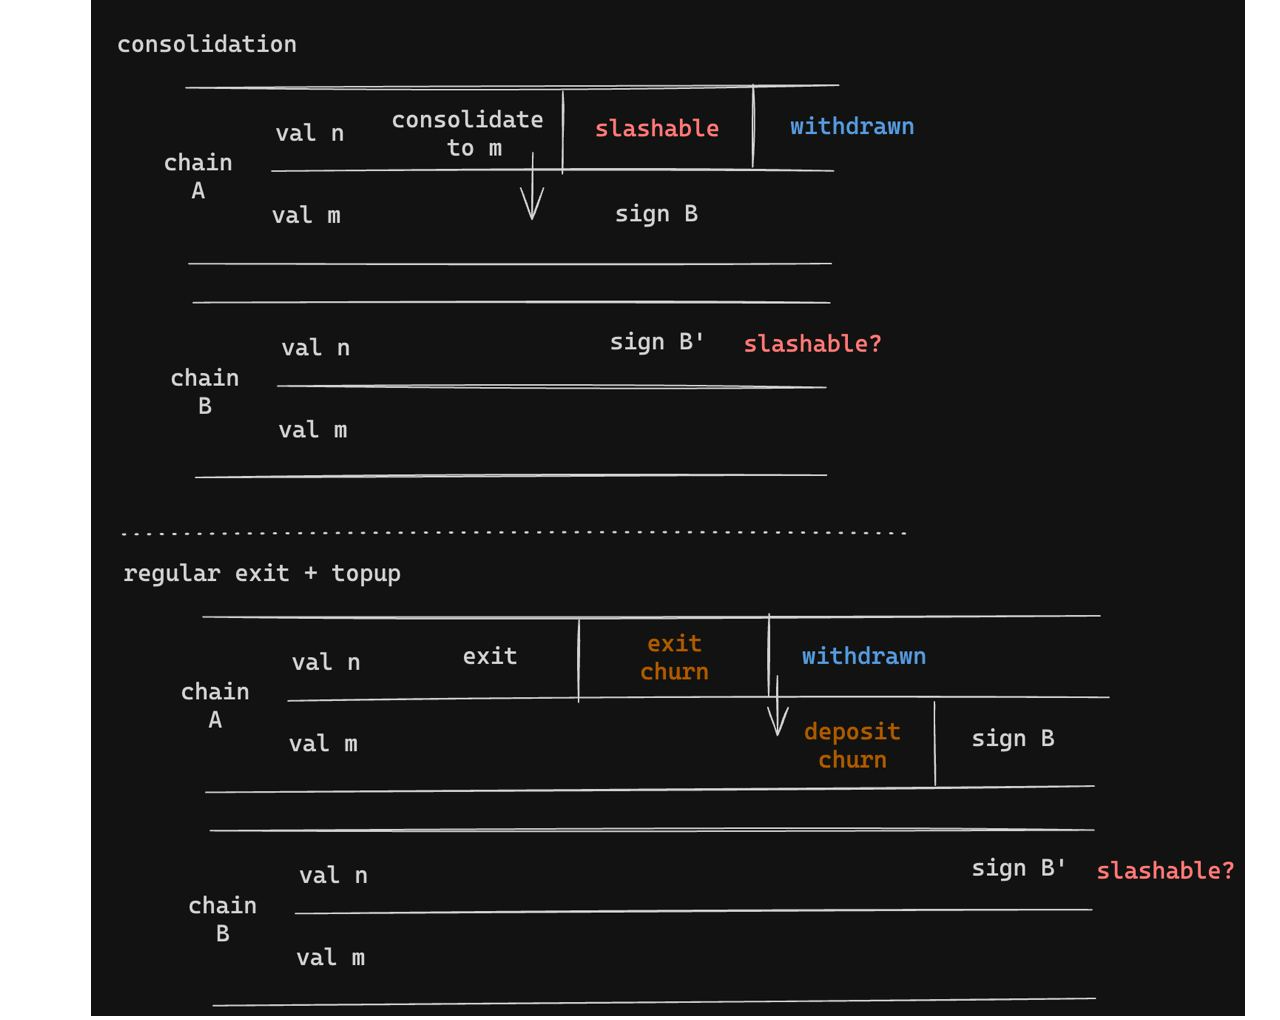
\includegraphics[width=0.7\linewidth]{images/francesco1}
\caption{A fork where consolidation is yet to occur and one where it has happened}
\label{fig:francesco1}
\end{center}
\end{figure}

\noindent
\textbf{Scenario 2 - fork during consolidation} \\
In figure~\ref{fig:francesco1} we see that validator \textit{n} consolidates to validator \textit{m} on chain \textit{A}, but not on chain \textit{B}. 

Validator \textit{n} then signs two different blocks at the same slot, or does surround voting, in a way that is not deemed to be slashable in the existing consolidation \gls{pr}. Based on this potential scenario, Francesco wondered if it would be that complicated to enable slashing ``across consolidations''.

Mikhail replied that this would be possible, providing that chain \textit{B} is aware that the consolidation happened on chain \textit{A}. Moreover, a slasher would need to resolve the final consolidation index in order to detect a new source of slashable offences between the source and target of consolidated validators.

Mikhail suggested three options to enable slashing across consolidations:
\begin{enumerate}
\item pass the consolidating stake through the activation churn.\\
\\
Bypassing the exit churn would be the improvement for stakers and a consolidation to be reverted if the source is slashed before the \gls{eb} was fully activated, without the necessity to make the target liable for the source's slashings.\\
Mikhail feels that this option is more natural from the protocol perspective. Consolidating via churn when the queue is empty means it will be 4 epochs, instead of 2 epochs to wait for consolidation to be finalised. However, Francesco pointed out that a large amount of consolidations would require weeks or months of churn.  Nonetheless, Mikhail does not expect pools to consolidate much faster than allowed by the churn due to the inherent risks. The concern is that pools would be reluctant to consolidate via churn due to lost revenue. 

\item finalise consolidation on-chain before activating a consolidated balance. This is akin to waiting for \textit{activation\_eligibility\_epoch} to be finalised. \\
\\
This is Mikhail's preferred option, with the addition of improving the slasher's design.
\item accompanying the slashing message with the consolidation from another chain.
\end{enumerate}

Mikhail summarised the proposed slashing rule for a consolidation event is as follows: \\
\noindent
Resolve the final target validator and slash the whole consolidation chain: the source, interim targets and the final target.

From the perspective of the slasher, the slashable offence occurs whenever \textit{consolidated\_to} is changed on any of the observable forks. 


